
\section{Problem Statement}\label{sec:state_of_art}

% ==============================
% Problem Statement Chapter
% ==============================

% Highlight the issue of inter-observer variability and the need for
% robust models that can learn from inconsistent labels.

Throughout the development of medical technology and \gls{CAD}, the
task of \gls{ISS} has become a crucial step in delivering precise diagnosis
and treatment planning \cite{Giri_Bhatia_2024}. Particularly, in the
area of histopathological studies, the usage of Whole Slide Images
(\gls{WSI}) is rather common since this method delivers high quality
imaging and allows for the diagnosis of diseases like cancer
\cite{YujiaEtAl2024}.

\gls{ISS} task consists of assigning a label to each pixel
in an image according to the object it belongs to. Accurate
segmentation is essential for the development of \gls{CAD} systems,
as it allows the identification of regions of interest (\gls{ROI}) in
the images, which can be used to detect and classify diseases and
hence, treatment planning \cite{Sarvamangala2022}. However, modern computational
solutions for \gls{ISS} tasks involve the use of deep learning, which
mostly rely large amounts of labeled data to train the models
on supervised learning techniques. This means that the model is trained on
a dataset with ground-truth labels, which are assumed to be correct
and consistent across all samples. In practice, this assumption is
often violated due to the high technical complexity of labeling these
segments \footnote{compared to a more trivial task like image classification
on ordinary an well known classes like MNIST}.

% The Multiple-Labelers Challenge
% Detail how medical images often require annotations from multiple
% experts with varying levels of expertise.
% Discuss common issues such as random errors (accidental mistakes)
% and expertise errors (systematic biases due to limited knowledge).
% Reference existing approaches that either require ground-truth
% labels or additional supervision to model labeler performance explicitly.

The process of labeling medical images is often managed with the help of
specialized software tools that allow the annotators to draw the
regions, delivering an standard format for the labeled
masks \cite{Habis2024}.
Despite the help of these tools, the labeling process in \gls{WSI} can have high
costs, as it requires long hours of work from specialized personnel.
Because of cost constraints in many medical institutions, the labeling processes
is often done by multiple labelers with varying levels of expertise, equalizing
the cost of the labeling process. However, this strategy can lead to
inconsistent labels, as the consensus between the labelers may not be
exact due to the diversity in depth of knowledge and experience of
the labelers \cite{XuYan2024}.
These inconsistencies are mostly represented in the subsections
\ref{subsec:expertise_levels} and \ref{subsec:technical_constraints}.

\subsection{Variability in Expertise Levels}\label{subsec:expertise_levels}

One of the primary sources of inter-observer variability in medical
image segmentation is the difference in expertise levels among
annotators \cite{Lopez2023}. Experienced radiologists and
pathologists tend to produce highly precise annotations, whereas
novice labelers may introduce systematic biases due to their limited
familiarity with subtle image features. Studies have demonstrated
that annotation accuracy \textit{tends} to improve with experience, yet medical
institutions often rely on a mix of annotators to manage costs and
workload distribution \cite{LuEtAl2023}.

The training background of annotators and institutional guidelines
play a crucial role in shaping labeling practices. Different medical
schools and hospitals may adopt distinct segmentation protocols,
leading to inconsistencies when datasets are combined from multiple
sources \cite{Lopez2023}. For example, some institutions may emphasize
conservative delineation of tumor boundaries, while others adopt a
more inclusive approach. Such variations contribute to systematic
biases in medical image datasets \cite{BanerjeeEtAl2025}.

Medical images frequently contain structures with ambiguous
boundaries, making segmentation inherently subjective. For instance,
tumor margins in histopathological slides may not have well-defined
edges, leading to variations in how different annotators delineate
the regions of interest \cite{Carmo2025}. These discrepancies arise not only
from technical expertise but also from differences in perception and
interpretation.

\subsection{Technical Constraints and Image
Quality}\label{subsec:technical_constraints}

Technical constraints in medical imaging, such as resolution
differences, noise levels, and contrast variations, can significantly
impact segmentation accuracy. Lower-resolution images may obscure
fine structures, leading to inconsistencies in boundary delineation
\cite{ZhouEtAl2024}.

When combined with long sessions, bad images might
also increase the cognitive load of the annotators, leading to
fatigue and reduced precision in labeling \cite{KimYujinAndLee2024}.
This is particularly relevant in histopathological studies, where the
staining process and tissue preparation can introduce color
variations and artifacts that affect image quality, even if the same scanning
equipment is used \cite{Karthikeyan2023}.

\begin{figure}
  \centering
  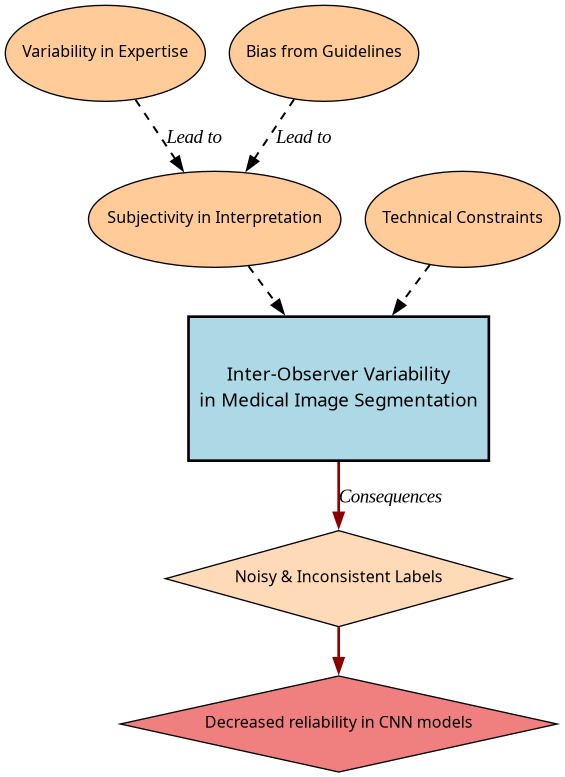
\includegraphics[width=0.7\textwidth]{Cap1/Figures/problem_statement_diagram.png}
  \caption{Summary diagram for problem Statement}
  \label{fig:problem_statement_diagram}
\end{figure}

\subsection{Research Question}

% Formulate the research question that addresses the need for a
% learning approach that can adapt to inconsistent labels.
% Emphasize the importance of developing a model that can infer
% labeler performance without explicit supervision.
% Provide a brief overview of the proposed solution and its potential
% impact on medical image analysis.

Given the challenges posed by inconsistent labels in medical image
segmentation, this work aims to address the following research
question:

\researchquestion{How can we develop a learning approach for
  \gls{ISS} tasks in medical images that can adapt to inconsistent
  labels without requiring explicit supervision of labeler
  performance? Can such approach face problems related to the
  variability in expertise levels and technical constraints while preserving
interpretability, generalization and computational efficiency?}